\documentclass[t,12pt]{beamer}

%liste des packages utilsé
\usepackage[T1]{fontenc}
\usepackage[french]{babel}
\usepackage[utf8]{inputenc}
\usepackage{graphicx}
\usepackage{pslatex}

%definition d'une couleur pour les titres
\definecolor{grisbleu}{rgb}{0,0,153}


%definition du thème 1
\useoutertheme[height=0pt,left]{sidebar}
\usecolortheme{seahorse}
\setbeamercolor*{titlelike}{parent=structure}
\useinnertheme{circles}
\setbeamertemplate{frametitle}[default][right]

%definition du thème 2
%\useinnertheme[shadow=true]{rounded}
%\useoutertheme{shadow}
%\usecolortheme{orchid}
%\usecolortheme{whale}



% contenu de la page de titre
\title{Projet tuteuré}
\subtitle{UFWI}
\author{Simon BAROTTE, Valentin FROLICH, Cyril PIERRÉ, Maxime ROBIN}

\begin{document}

%------- page de titre --------
\frame{\titlepage}

% --------- Sommaire ---------

\begin{frame}{Sommaire}
	\tableofcontents[]       %genere un somaire automatique (avec les \section)
\end{frame} 

%-----page Objectif-----------
%---------------------------------------------------------------------------------------------------
%------------ Maxime Robin -------------------------------------------------------------------------
%---------------------------------------------------------------------------------------------------
\section{Introduction}  
  \subsection{Présentation}                                            
    \begin{frame}{Présentation}                                              
	    \begin{block}{Historique}
        \begin{itemize}  
	        \item La première version publique de NuFW par EdenWall est sortie le 01 septembre 2003.
	        \item Le 18 août 2011, liquidation de NuFW et reprise du projet par la communauté (Ufwi).
        \end{itemize} 
      \end{block}
      \pause
      \begin{block}{Présentation}
        \begin{itemize}  
	        \item Surveillance de l'activité réseau des serveurs.
	        \item Paquets signés.
	        \item Module de surveillance (logs).
          \item Identifier les utilisateurs par une authentification unique.
        \end{itemize} 
      \end{block}
    \end{frame} 

  \subsection{Algorithme}
    \begin{frame}{Algorithme}
	    \begin{center}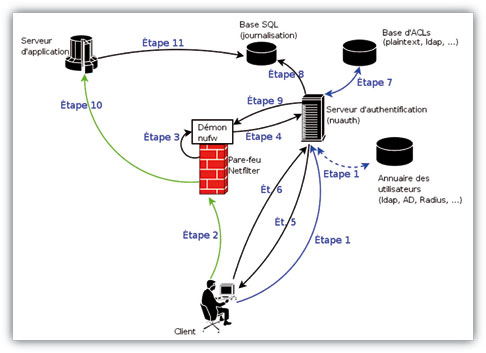
\includegraphics[width=7cm,height=6.5cm]{images/algo.jpg}\end{center}
    \end{frame}                                                      

%---------------------------------------------------------------------------------------------------  

\section{Modules}                                                   
\begin{frame}{Modules}
    \begin{itemize}                                                 
	\item Authentification
	\newline
	\item Filtred
	\newline
	\item Rcpd
	\newline
	\item Client
\end{itemize}
\end{frame}                                                         

	  \subsection{Authentification}
	  \begin{frame}{Authentification}                                                         %définit le debut de la page
		\begin{block}{Présentation}
		  \begin{itemize}
		    \item Daemon principale
		    \item Gère toutes les authentifications	    
	    \end{itemize}
		\end{block}
		
		\begin{block}{Configuration}
		  \begin{itemize}
		    \item Module ldap, plaintext
		    \item Journalisation des connexions
		    \item Certificats		    
	    \end{itemize}
		\end{block}
		
		\begin{itemize}
		\item Fonctionnement de l'authentification
	  \end{itemize}
	  \end{frame} 


	  \begin{frame}{Authentification}                                                         %définit le debut de la page
		  \begin{center}
		    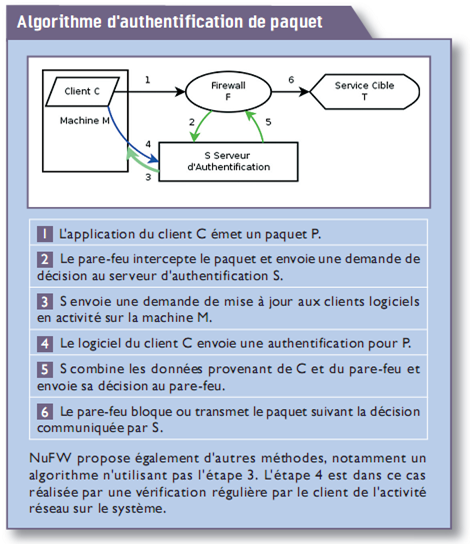
\includegraphics[width=6cm,height=6.5cm]{images/auth.png}
		  \end{center}
	  \end{frame} 

	  \subsection{Filtred}
	  \begin{frame}{Filtred}                                                         %définit le debut de la page
	      \begin{itemize}                                                   %definie une liste
		      \item Présentation
		      \end{itemize}
		\begin{block}{Fonctionnalités}
			\begin{itemize}
		    \item Filtre le trafic
		    \item Module de surveillance
		    \item Contribue à la surveillance réseau
		    \item Marque chaque paquet avec un ID unique
	    \end{itemize}
		\end{block}
  
    \begin{itemize}
		\item Fichier de configuration
	  \end{itemize}
	  \end{frame} 

	  \subsection{Rcpd}
	  \begin{frame}{Rcpd}                                                         %définit le debut de la page
	                                                         %definie une liste
		\begin{block}{Présentation}
		  \begin{itemize}
		    \item Manager
		    
	    \end{itemize}
		\end{block}
		
		\begin{block}{Types d'authentification}
		\begin{itemize}
		  \item alwaysok
      \item alwaysno
      \item basicdict
      \item file
      \item ldap
	  \end{itemize}
    \end{block}
    
    \begin{itemize}
	    \item Composants et servies
	    \item Tâches planifiées
	  \end{itemize}
	  \end{frame} 

	  \subsection{Client}
	  \begin{frame}{Client}                                                         %définit le debut de la page
	      \begin{itemize}                                                   %definie une liste
		\item Présentation
		\newline
		\item Différent client disponnible
		\newline
		\item Multi-plateformes
		\newline
		\begin{center}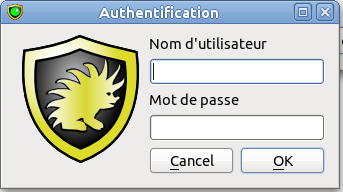
\includegraphics[width=4cm,height=3cm]{images/nuapp.png}\end{center}
	  \end{itemize}
	  \end{frame} 

\section{Comparaison}                                                    %utilisé pour la generation du sommaire
\begin{frame}{Comparaison}                                                         %définit le debut de la page
    \begin{itemize}                                                   %definie une liste
	\item Différentes solutions de pare feu
  \begin{itemize}
    \item AuthPF
    \item NUFW
    \item Cyberoam
    \item CheckPoint
  \end{itemize}
	\pause
	\item Installation, mise en oeuvre
	\item Modularité
  \item Sécutité
  \item Intérêts
\end{itemize}
\end{frame}                                                            %définit la fin de la page


\section{Problèmes et Conclusion}                                                    %utilisé pour la generation du sommaire
\begin{frame}{Problèmes et Conclusion}                                                         %définit le debut de la page
    \begin{itemize}                                                   %definie une liste
	\item Problèmes lors de l'installation
	\item Problèmes de configuration
	\item Conclusion
\end{itemize}
\end{frame}                                                            %définit la fin de la page
	\subsection{Problèmes lors de l'installation}
		\begin{frame}{Problèmes lors de l'installation}                    %définit le debut de la page
		\begin{itemize}
			\item Problèmes de dépendances
			\newline
			\item Problèmes d'obsolèscence
			\newline		
			\item Problème dans le code
			\newline
			\item Peu de documentation
		\end{itemize}
		\end{frame}

	\subsection{Problèmes de configuration}
		\begin{frame}{Problèmes de configuration}                        %définit le debut de la page
		\begin{itemize}
			\item Problèmes de librairies
			\newline
			\newline
			\item Problèmes de certificats
		\end{itemize}
		\end{frame}


	\subsection{Conclusion}
		\begin{frame}{Conclusion}                                                         %définit le debut de la page
		\begin{itemize}
			\item Projet Libre
			\newline
			\item Projet ayant sa place dans la sécurité des entreprises
			\newline
			\item Logiciels modulables et multi-plateformes
			\newline
			\item Des lacunes 
		\end{itemize}
		\end{frame}


\end {document}
